\documentclass[12pt, a4paper]{report}
\usepackage[left=3.5cm, right=2.5cm]{geometry}

\usepackage[utf8]{inputenc}

\usepackage{graphicx}
\usepackage{epstopdf}
\usepackage{float}
\usepackage{pdfpages}
\usepackage{listings}
\usepackage{xcolor}
\usepackage{amsmath}

\lstset { %
    language=C++,
    frame=tb, % draw a frame at the top and bottom of the code block
    backgroundcolor=\color{black!5}, % set backgroundcolor
    basicstyle=\footnotesize,% basic font setting
    numbers=left, % display line numbers on the left
    tabsize=4, % tab space width
    breaklines=true,
}

\usepackage{tikz-cd}
\usetikzlibrary{arrows.meta, arrows, decorations.markings}
\usetikzlibrary{positioning, automata}
\usetikzlibrary{fit}
\usetikzlibrary{decorations.pathreplacing}

\usepackage{caption}

\usepackage{placeins}

\let\Oldsection\section
\renewcommand{\section}{\FloatBarrier\Oldsection}

\let\Oldsubsection\subsection
\renewcommand{\subsection}{\FloatBarrier\Oldsubsection}

\let\Oldsubsubsection\subsubsection
\renewcommand{\subsubsection}{\FloatBarrier\Oldsubsubsection}


\title{
	{Performance Evaluation of Round Robin CQI based Cellular Network}\\
	{\large Università di Pisa\vspace{1cm}}\\
	{
\includegraphics[scale=.5]{images/cherubino_pant541.eps}}
}
\author{Antonio Le Caldare, Vincenzo Consales, Vincent Della Corte}
\date{year 2017/2018}


\begin{document}
\maketitle

\tableofcontents

\chapter{Modelling}
\section{Introduction}
In these paragraph we describe how we modeled the Celluar Network described in the specifications.
\begin{itemize}
   \item \textbf{A Web Server}, which generates data in the form of packets to be trasmitted to users. For our pourposes we have defined the class \texttt{UserPackets} which includes a \texttt{start\_time} field and its interface (named \texttt{UserPacket\_m}) includes a getter/setter method to update this field.
   
   The size of each packet is an integer RV \(\sim U(3,75)\), since the service demand has to be uniform and consistent with the frame size. Moreover the packet interarrival time to the antenna has to be an exponential RV, so each packet is generated properly to satisfy this requirements.

   \item \textbf{An Antenna}, which has FIFO queue for each user. Packets received form \textbf{Web Servers} are stored inside queues and then are sent in a unicast way according to the Round Robin policy (which is described in the next section). 
   
   \item \textbf{A Mobile Station}, which personifies a generic user connected to the antenna. On each timeslot it sends a channel quality indicator (CQI), which is a number between 1 and 15 that define the number of bytes the antenna can pack into a Resource Block (RB).
   
   CQIs are integer RVs generated according the following scenarios:
   
   \begin{enumerate} 
    \item Uniform, each user generates a RV \(\sim U(1,15)\)
    \item Binomial, each user generates a RV \(\sim Bin(n,p_i)\), where \(n\) is the number of users, and \( 0<p_i<1\) depends on the user i.
    \end{enumerate} 
\end{itemize}
To build our model and to run rimulations we used the framework \textbf{OMNeT++ v5}, so each item described before is defined by a \texttt{*.ned} file.
Each \texttt{Mobile Station} computes some statistics: slotted throughput (related to each time slot) and response time of received packets. The \texttt{Antenna} compute also statistics about the frame filling, which we will describe later.

The \texttt{CellularNetwork.ned} file shows how the previous modules are connected to obtain the network. Since frames are sent in a unicast way, there are multiple instances of the Web Server module, one for each Mobile Station, seeded in a different way in order to have IID RV.

The obtained network, by setting \(n=10\), is the following: 
\begin{figure}[H]
  \centering
  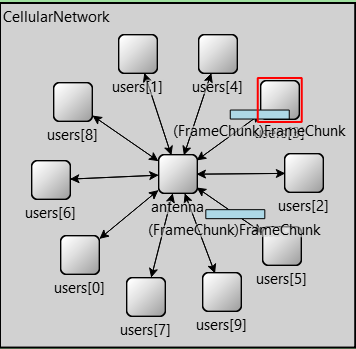
\includegraphics{images/network_simulations}
  \caption{Simulated Network (omnet++)}
  \label{fig:simulated_network}
\end{figure}

\section{Frame Chunks}
  Packets are delivered to users by enveloping that inside RBs. As requested by specifications \(RBsize\textsubscript{i,t\textsubscript{j}}=f(CQI\textsubscript{i,t\textsubscript{j}})\) where \(i\) is index of \textit{user}, and \(t\textsubscript{j}\) is index of \textit{timeslot}.
  To do that, the scheduler receives CQIs from the \texttt{Mobile Stations} at beginnig of each time slot, then compute every \(RBsize\textsubscript{i,t\textsubscript{j}}\) and fills the frame according to scheduling policy. Note that a frame can carry RBs for different users so, generally speaking, a frame in a specific time slot \(t\textsubscript{j}\) can have RBs of different size. To cope these requirements we defined a new module \texttt{Frame Chunk} wich groups all RBs addressed to a specific \texttt{Mobile Station}. By introducing this module we can consider a frame as a collection of \texttt{Frame Chunks}. To deliver the whole frame we must send each \texttt{Frame Chunk} to its user in a unicast way.

\section{Schedulers}
  In this section we will analyze the frame filling policy wich are defined in the module \texttt{Scheduler}.
  Let's consider a user \(0\leq i < n\). Starting from user \(i\), the scheduler allocates a new \texttt{Frame Chunk} and fills it with packets taken from the \texttt{FIFOQueue\textsubscript{i}}. A \texttt{Frame Chunk} is considered full if it contains 25 RBs because it corresponds to the whole frame. At the next time slot will be served the user \((i+1)\textnormal{mod }n\). If the frame is not full the scheduler must allocate others \texttt{Frame Chunks} in order to fill the residual space using one of the two following policies. 

\begin{itemize}
%\subsection{Round-Robin Frame Fill}
  \item \textbf{Round-Robin Frame Fill}
  The residual space  in the frame is filled by considering the following \texttt{FIFOQueues\textsubscript{j}} \(j \in \{ (i+1)\textnormal{mod } n,(i+2)\textnormal{mod }n,\ldots \} \)
%\subsection{Best CQI based Frame Fill}
  \item \textbf{Best CQI based Frame Fill}
   The residual space in the frame is filled by considering the users with the best(highest) CQI in a decreasing order. In the case of \(CQI\textsubscript{i}=CQI\textsubscript{j} \mid i < j\) is selected the user \(i\).
\end{itemize}
We will analyze the effect of both policy to performace regarding the throughput and the response time for each user with varying workloads.

\section{Constants}
In the following chapters, if not different specified, we will consider this constants.
\begin{itemize}
\item \textbf{Number of resource block}, \(\#RB = 25\)
\item \textbf{Number of users}, \(n = 10\)
\item \textbf{Max RB size}, \(RBsize\textsubscript{max} = 93\)
\item \textbf{Max packet size}, \(packetsize\textsubscript{max} = 75\)
\item \textbf{Timeslot period}, \(T\textsubscript{slot} = 1\textnormal{ms}\)
\item \textbf{Number of repetions}, \(\#REP = 10\)
\item \textbf{Simulation time}, \(simtime = 1 \textnormal{min}\)
\end{itemize}
\chapter{Simulation}

\section{Introduction}
How we said in the previous chapter we built the model inside the framework \textbf{OMNeT++ v5}. The definition of network \textit{(CellularNetwork.ned)} and their components can be found in the directory \textit{RRCellNet/src}. We decided to analyze it when 10 \texttt{Mobile Stations} are connected to the \texttt{Antenna}. In order to simplify the model we represented the network with a \textit{Star Topology}. \texttt{Mobile Stations} receive packets through unicast channel \texttt{without transmission delay}.

We recall that \texttt{Web Servers} are sources of packets addressed to \texttt{Mobile Stations}. In order to have true random and independent arrivals to \texttt{Antenna} we need a 10 RNG, one for each \texttt{Web Server}. We also need RNG to generate packets with random size so others 10 RNG are neeeded. We need also a RNG for each \texttt{Mobile Station} in order to generate random CQIs at each timeslot. Overall the model requires 30 RNGs each of them initialized with a different seed in order to have independent pseudo-random variables. The seed-set is changed at every repetition to have different independent experiments. At the end of all repetions the results are aggregated by computing the mean and 95\% confidence interval. 

Let's consider for example the mean throughput for a rate \(\lambda^{*}\). By running each repetition we get the values \(X_{1},X_{2},\ldots X_{10}\). \(X_{i}\) is a random variable which represents the mean throughput for the repetition \(i\). By the CLT theorem we can say that \(X_{i}\) is a normal RV since it is obtained by summing up a huge number of \textit{slotted throughput}. We can estimate the mean \(\bar{X}\) and a 95\% confidence interval by using the \textit{Student's t distribution} because \(X_{i}\) are normal RV. 

\begin{align}
	\bar{X} &= \frac{X_{1}+X_{2}+\ldots+X_{10}}{10} \qquad S^{2} = \frac{1}{9}\sum_{i=1}^{10}(X_{i} - \bar{X})^{2} \\
	CI_{0.95} &= \left[\bar{X} - \frac{S}{\sqrt{10}}t_{0.025,9}, \: \bar{X} + \frac{S}{\sqrt{10}}t_{0.025,9}\right]
\end{align}

Similar consideration can be done for others quanties wich we will analyze during simulations. Once we have computed the mean \(\bar{X}\) and its confidence interval we can do a box plot for that quantity at varying workload \(\lambda\) as required by specifications. Data are exported from simulation to csv files through a bash script \textit{exportdata.sh} and plots are done through an R script \textit{analyze\_csv.r}. These script are both included in the directory \textit{RRCellNet/simulations}.

All parameters for simulations are summarized here and can be found in the file \textit{RRCellNet/simulations/omnetpp.ini}. We will use them in the following chapters unless otherwise specified.
\begin{itemize}
\item \textbf{Number of resource block}, \(\#RB = 25\)
\item \textbf{Number of users}, \(n = 10\)
\item \textbf{Number of RNG}, \(\#RNG = 30\)
\item \textbf{Max RB size}, \(RBsize\textsubscript{max} = 93\)
\item \textbf{Max packet size}, \(packetsize\textsubscript{max} = 75\)
\item \textbf{Timeslot period}, \(T\textsubscript{slot} = 1\textnormal{ms}\)
\item \textbf{Number of repetions}, \(\#REP = 10\)
\item \textbf{Simulation time}, \(ST = 60 \textnormal{s}\)
\item \textbf{Warmup period}, \(WP = 0.5 \textnormal{s}\)
\end{itemize}

\section{Warm-Up Period Estimation}
In the previous section we saw that the warm-up time is 0.5s, but we haven't specified yet how that value comes out.

In this section we will illustrate how we have estimated the length of the warm-up period. We followed this approach: for each scenario and for each user we plotted the graph of the throughput and the response time and then for each repetition we applied the sliding moving average and then we computed the sample mean of the latter in order to see how many time it was required to converge around that value.
We chosen the worst case among all of them, which graph is the following:

\begin{figure}[H]
  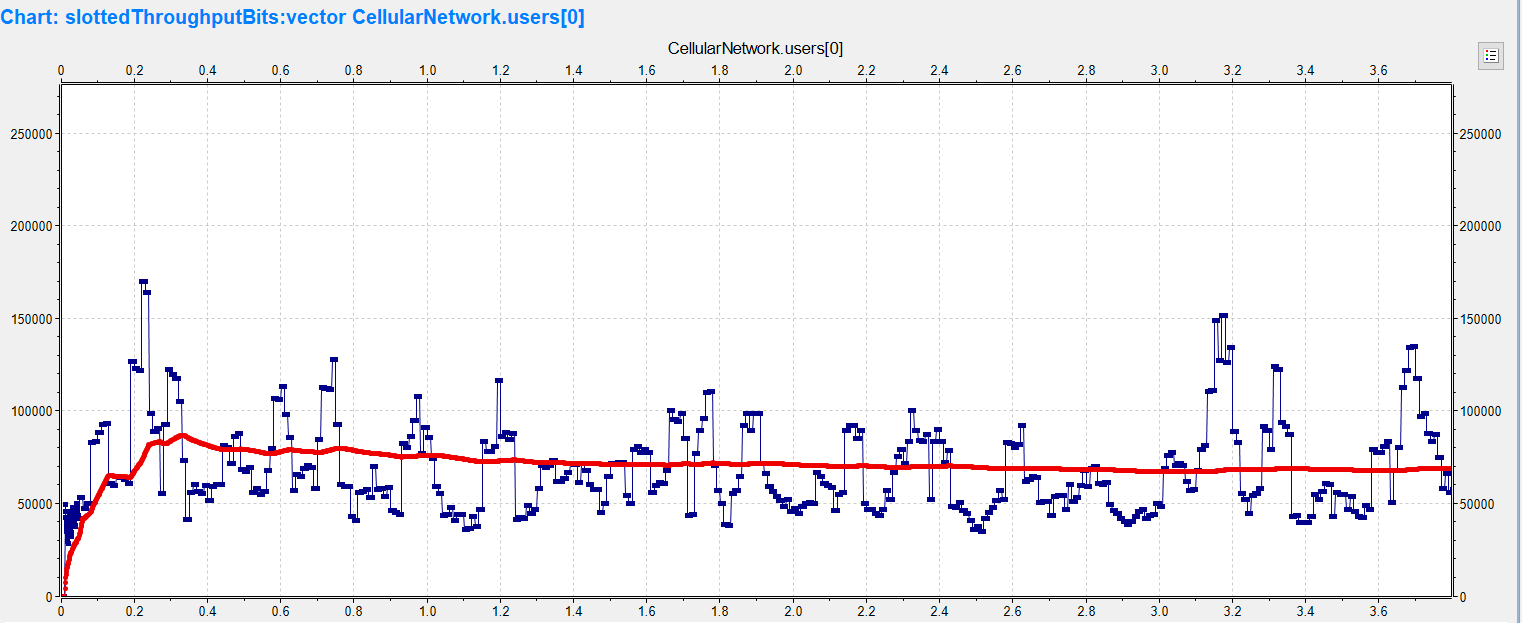
\includegraphics[width=1\textwidth]{images/binomial_user0_rate9_6_rep9}
  \caption{Worst Case for the Warm-Up period estimation}
  \label{fig:warm_up time}
\end{figure}

So we saw that in the worst case the graph converged to the sample mean after \textbf{0.5s} and we chosen that value as \textbf{warm-up time}.     
\chapter{Validation}

\section{Introduction}
After building our model inside the \textbf{OMNeT++} we can proceed with the simulation in order to analyze the quantities wich we are interested. First of all we will simulate the model in very simple cases in order to be sure it reproduces the system's behavior correctly. We decided to validate our model by \textit{removing randomness}. This choice allows us to do some easy computation by hand and to verify if the result of simulation is consistent with them. Our model will be considered a good replica of the system if it will pass all the \textit{validation tests}. During the validation we will use the first scheduler: \textbf{Round-Robin Frame Fill} because it generates simulation which are easier to analyze and to compare with analitical results.

\section{1\textsuperscript{st} test: fixed CQI, fixed \(\lambda\) rate, fixed packet size, 1 user}
In this test we just one \texttt{Mobile Station} connected to the antenna wich always generates the same CQI for each timeslot. Inside the \texttt{Web Server} the \(\lambda\) rate is fixed and also the packet size. This is a very simple system with deterministic arrivals and deterministic service demand. We can compute the traffic that \texttt{Web Server} sends to the antenna as 
\begin{equation} 
	th\textsubscript{in} = \frac{packetsize \times 8}{1/(1000\lambda)} \lbrack bps \rbrack 
\end{equation} 
If the system is in a stable state the output throughput and the input throughput must be equal. The maximum output throughput is the one we have by setting all parameters to maximum values. 
\begin{equation} 
	th\textsubscript{max} = \frac{\#RB \times RBsize\textsubscript{max} \times 8}{T\textsubscript{slot}} = \frac{25 \times 93 \times 8}{0.001} = 18.6 \textnormal{ Mbps}
\end{equation} 
We can derive very easily the \(\lambda\textsubscript{max}\) rate wich produces the max throughput allowed by antenna. 
\begin{equation}
	\lambda\textsubscript{max} = \frac{\#RB \times RBsize\textsubscript{max}}{1000 \times T\textsubscript{slot} \times packetsize\textsubscript{max}} = \frac{25 \times 93}{1000 \times 0.001 \times 75} = 31 \textnormal{ ms\textsuperscript{-1}} 
\end{equation}
For \( 0<\lambda<\lambda\textsubscript{max} \) the system is a stable state and so \(th\textsubscript{in} = th\textsubscript{out}\). For higher \(\lambda\) the FIFOQueue grows indefinitely because the frame is not able to carry as much data in a time slot.

Let's consider all the simulations with the following parameters:
\begin{itemize}
	\item \(\lambda \in \{1,2,\ldots,32\}\)
	\item \(packetsize=75\)
	\item \(CQI=15\)
\end{itemize}
  We can se in the graph a linear behavior regarding the throughput until the system is not saturated. Note that the response time for each packet is zero since there is no queueing until \(\lambda < \lambda\textsubscript{max}\) and grows indefinitely when the system saturates. This is not surprising since \(th\textsubscript{in} \propto \lambda\) when \(\lambda < \lambda\textsubscript{max}\) and packet's size is fixed.
\begin{figure}[H]
  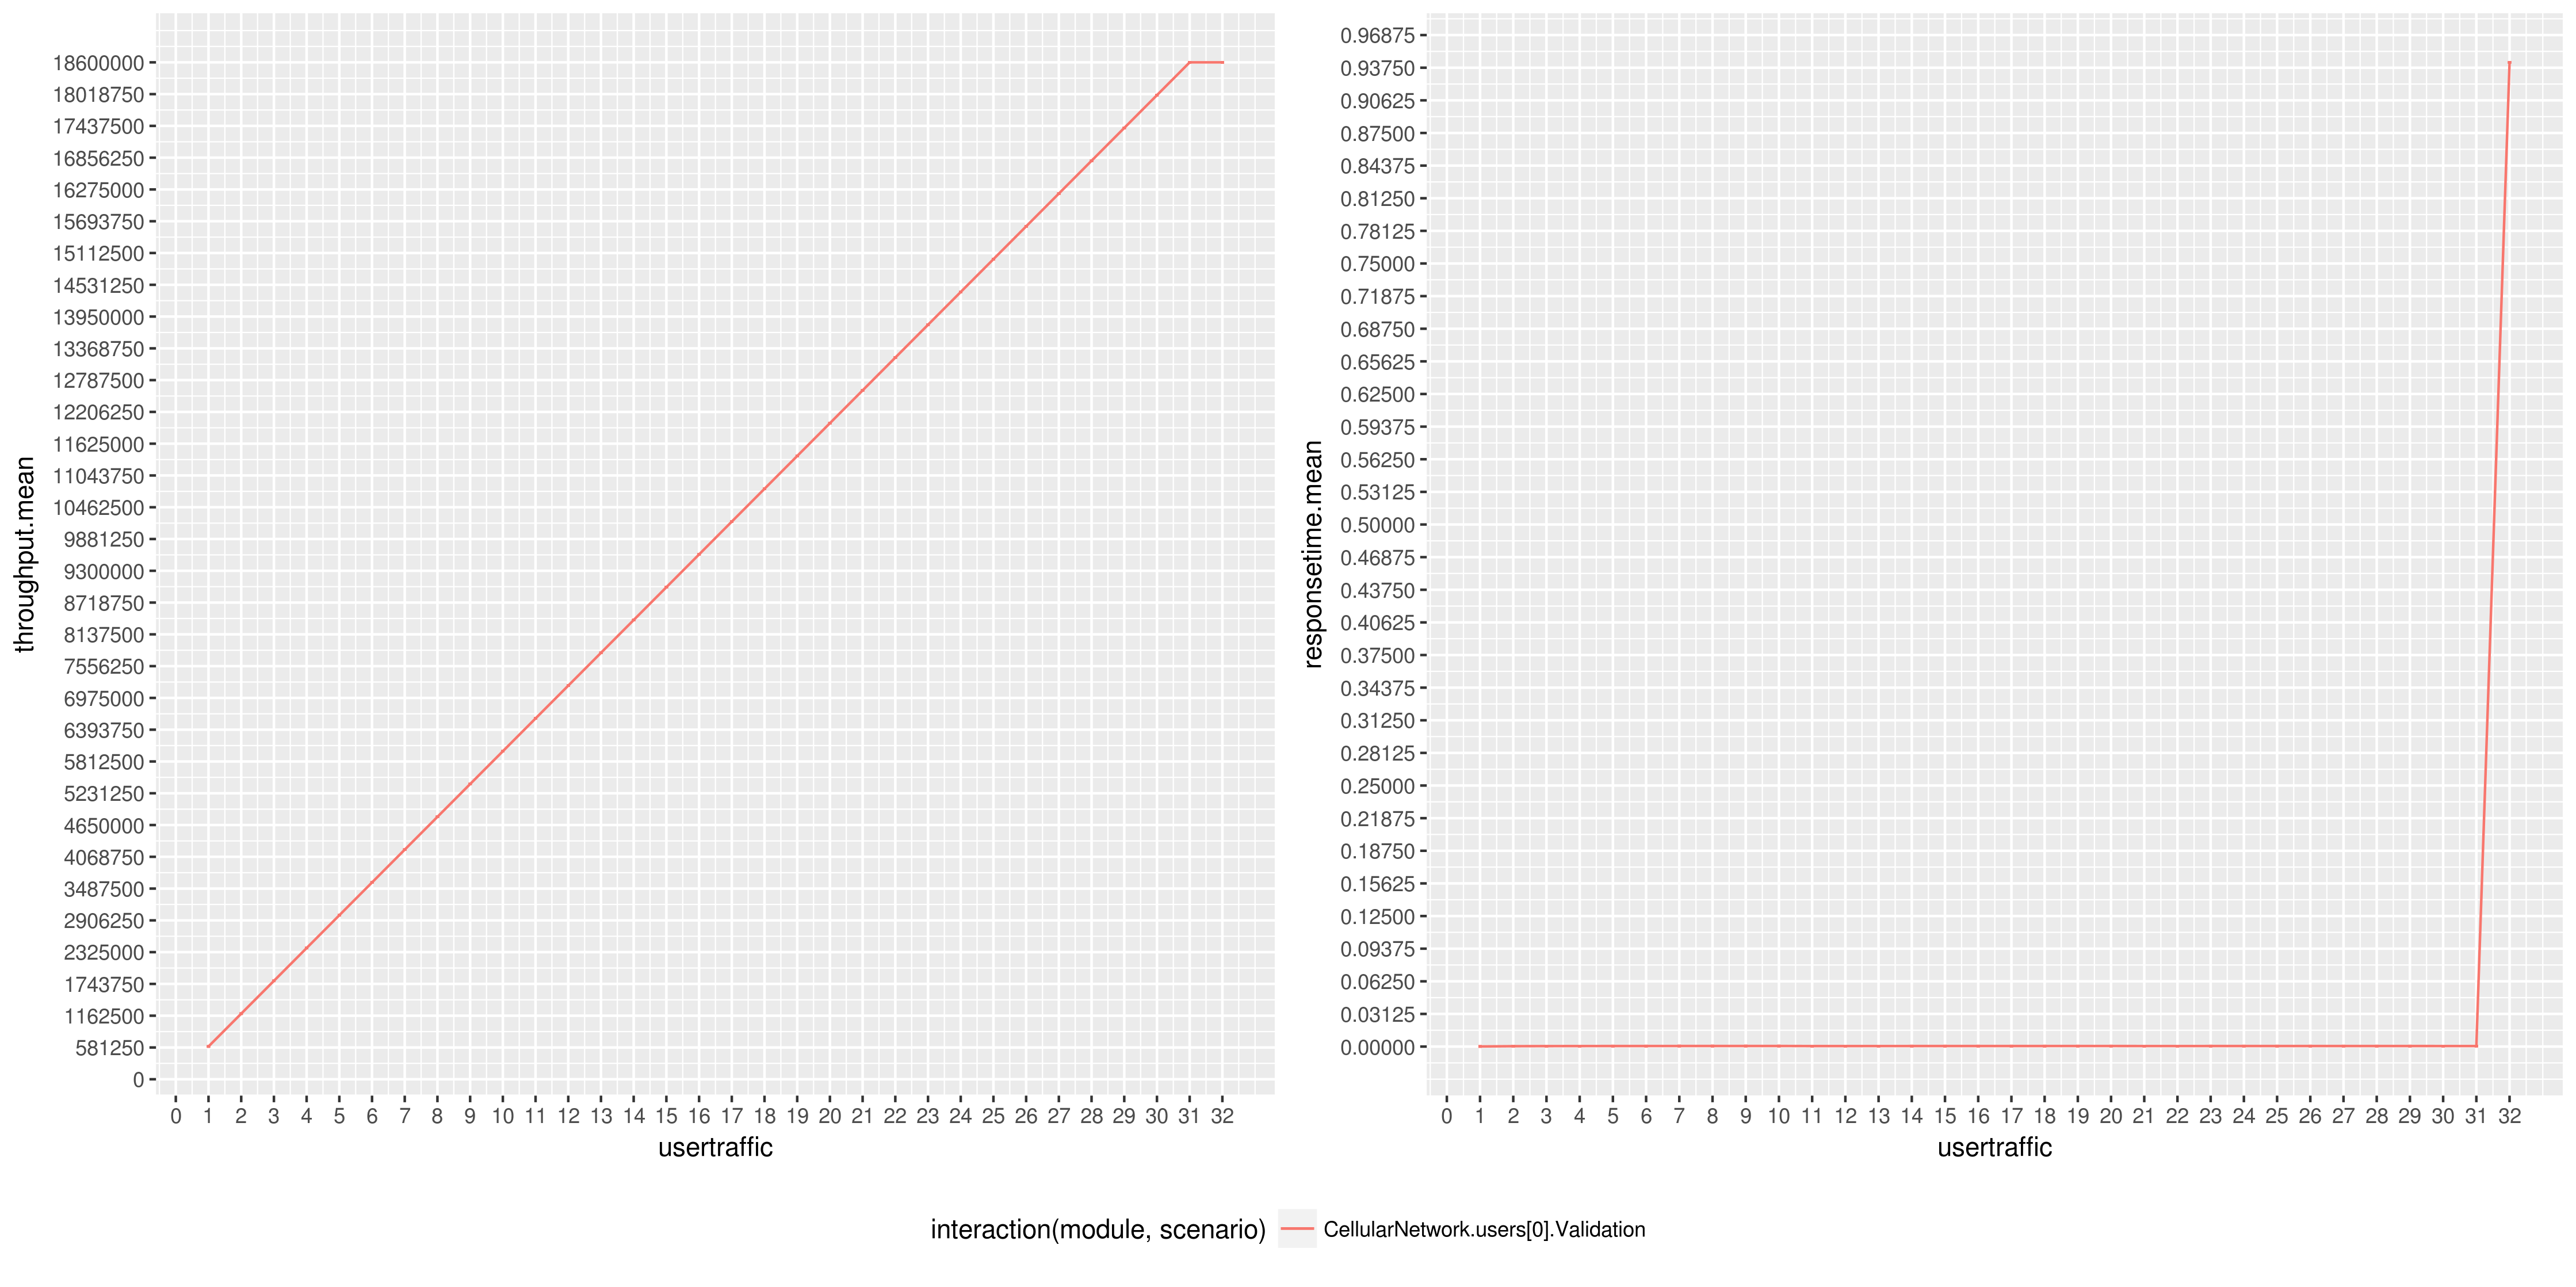
\includegraphics[width=1\textwidth]{images/plotvalidation}
  \caption{1st validation scenario: throughput, response time}
  \label{fig:1st validation scenario: throughput, response time}
\end{figure}

\section{2\textsuperscript{nd} test: fixed CQI, fixed \(\lambda\) rate, fixed packet size, 2 users}
In this test there are two \texttt{Mobile Stations} connected to antenna. As in the previous scenario all parameters are fixed. We have two indipendent flow of data from \texttt{Web Servers} to \texttt{Antenna} so the input throughtput could by computed as
\begin{equation} 
th\textsubscript{in} = \frac{packetsize\textsubscript{0} \times 8}{1/(1000\lambda\textsubscript{0})} + \frac{packetsize\textsubscript{1} \times 8}{1/(1000\lambda\textsubscript{1})}
\end{equation}
For these simulation we have chosen the following parameters:
\begin{itemize}
	\item \(packetsize_{0} = packetsize_{1} = 40\)
	\item \(CQI_{0} = 6\)
	\item \(CQI_{1} = 15\)
	\item \(\lambda = \lambda_{0} = \lambda_{1}\) and \(\lambda \in \{1,2,\ldots,32\}\)
\end{itemize}
We can compute the max \textit{slotted thorughput} for both users.
\begin{equation}
	\begin{split}
	slotth^{0}_{out} &= \frac{\#RB \times RBsize_{0} \times 8 }{T_s} = \frac{25 \times 20 \times 8}{0.001} = 4 \textnormal{ Mbps} \\ 
	slotth^{1}_{out} &= \frac{\#RB \times RBsize_{1} \times 8 }{T_s} = \frac{25 \times 93 \times 8}{0.001} = 18.6 \textnormal{ Mbps}
	\end{split}
\end{equation} 
\begin{figure}[H]
  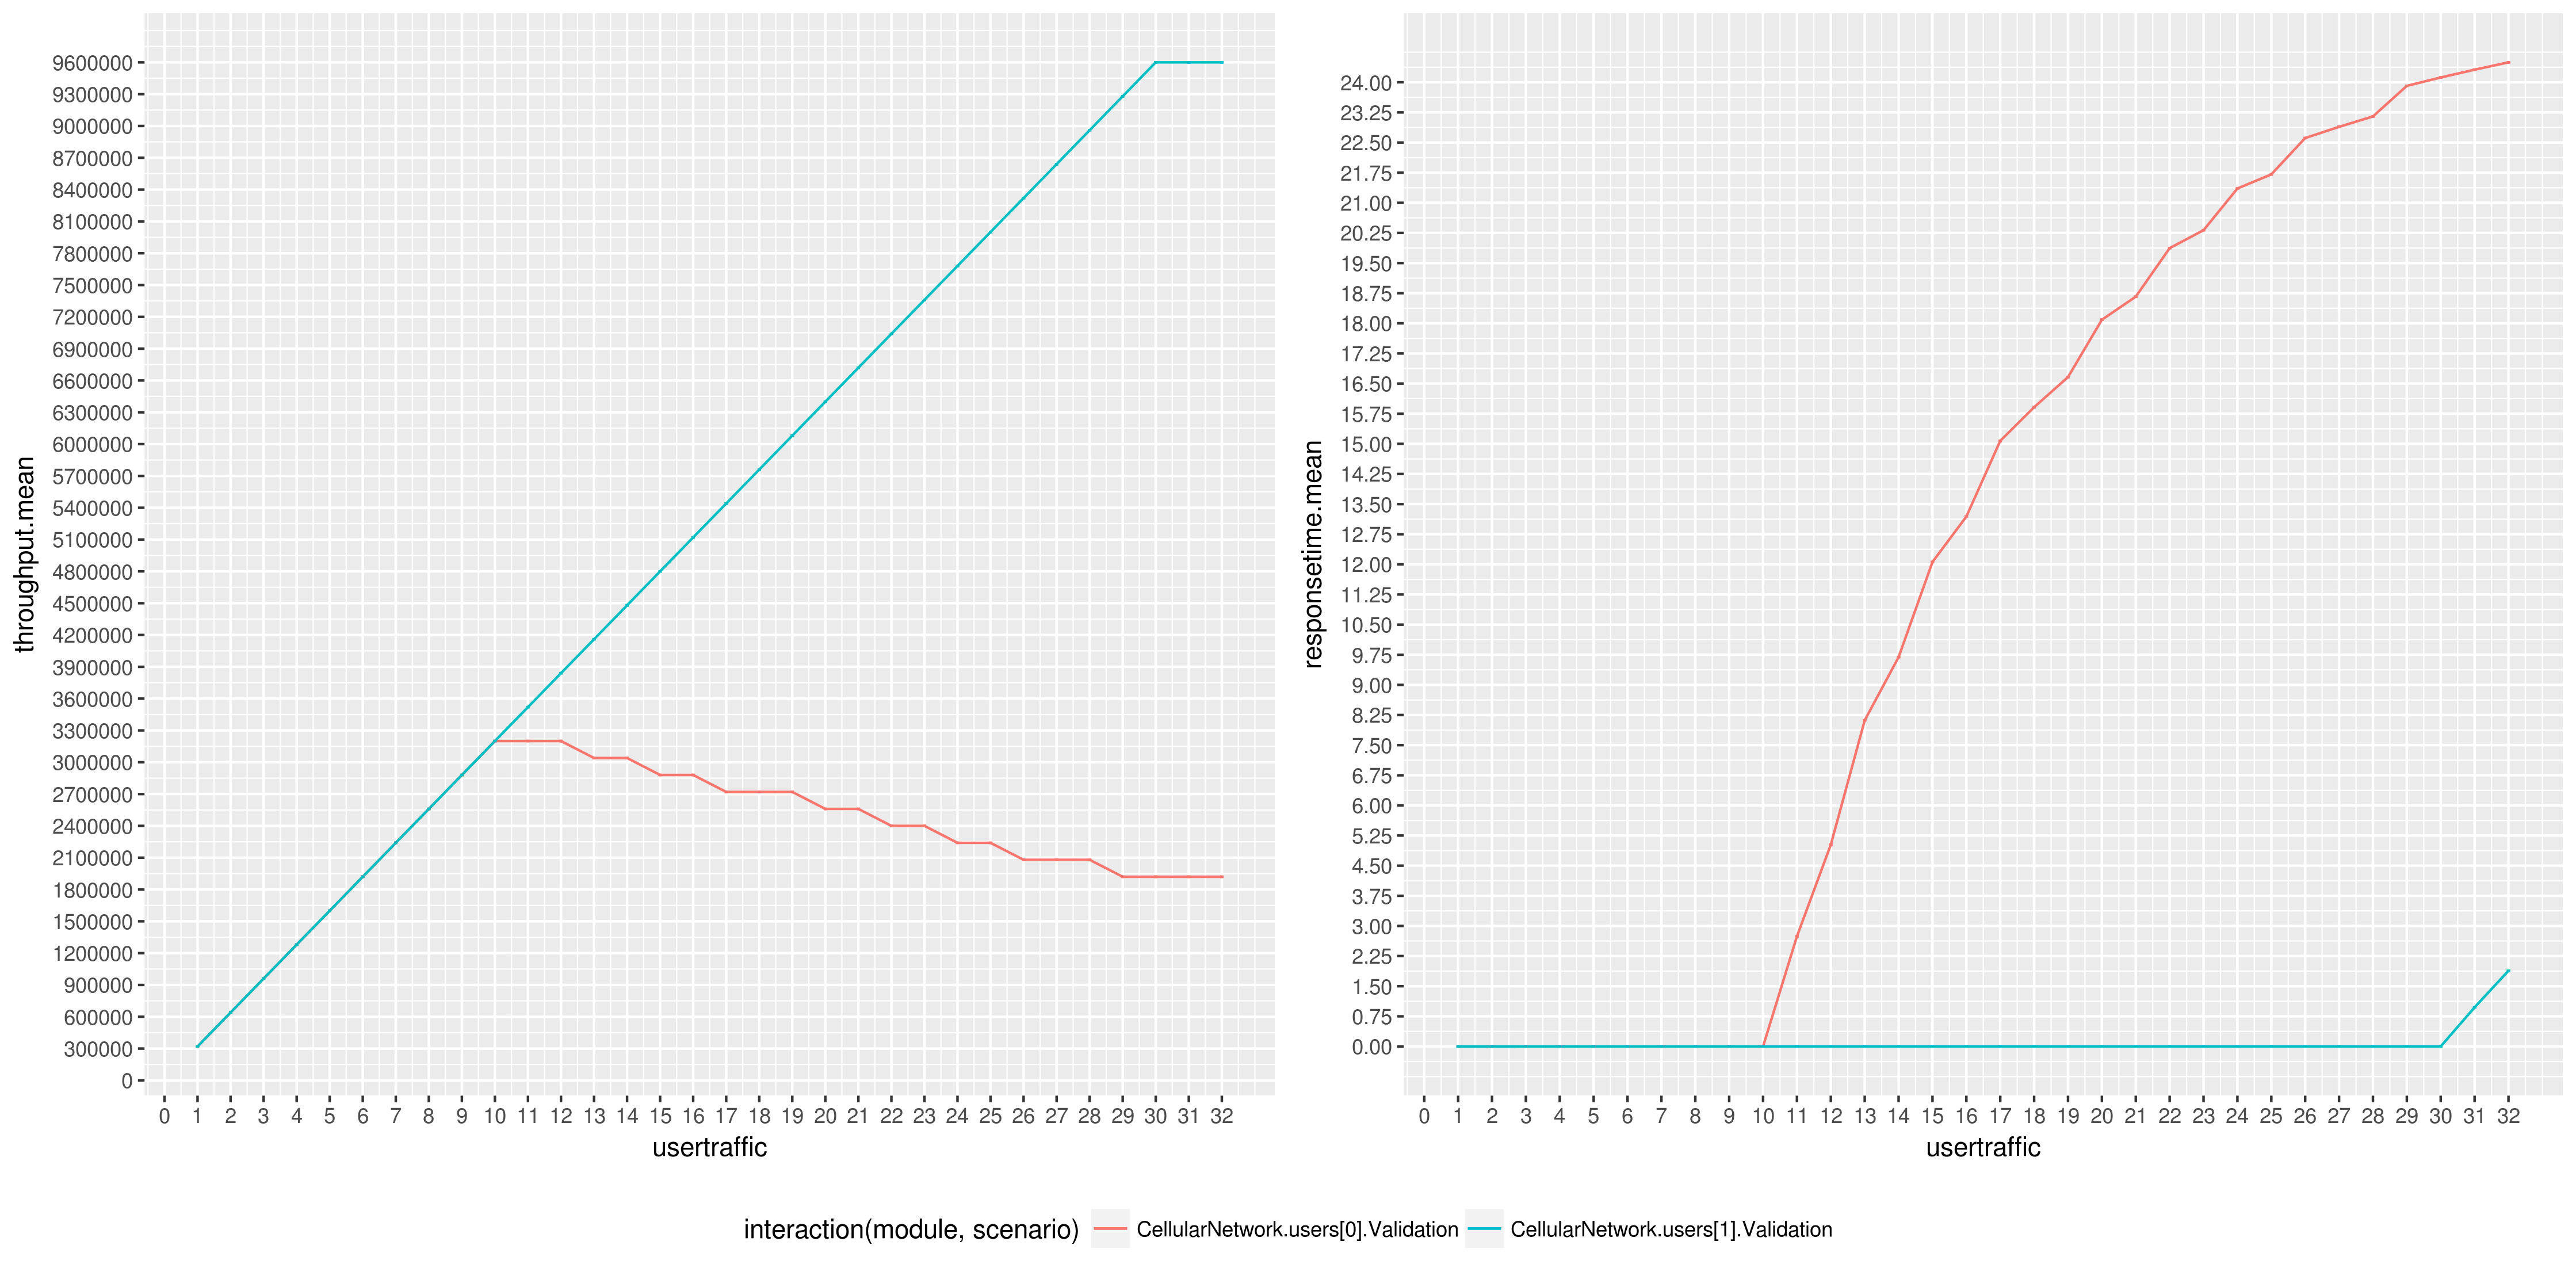
\includegraphics[width=1\textwidth]{images/plotvalidation2}
  \caption{2nd validation scenario: throughput, response time}
  \label{fig:2nd validation scenario: throughput, response time}
\end{figure}
At full load we expect that users compete to fill the frame. If the scheduler were fair, at full load, the average throughput would be \(th^{i}_{out} = (slotth^{i}_{out})/2\) since there are 2 users and the scheduler follow a round robin scheme, which is fair in principle. 

We see in the graph that throghput grows linear ad is equal for both users when \(1 \leq \lambda \leq 10 \). For \(\lambda > 10 \) the \texttt{Mobile User[0]} saturates, conversely \texttt{Mobile User[1]} continues to increase its throughput until it reaches saturation at \(\lambda = 30\).
When \(\lambda = 10 \) the input flow is \(th_{in}^{0} = th_{in}^{1} = (40 \times 8)/0.0001 = 3.2\textnormal{ Mbps}\) and this result could be seen also in the graph. Infact when \(\lambda \le 10 \) both users are in stable state so \(th_{in} = th_{out}\). We can see that, when \(\lambda\) increases the mean throughput approches to the half of slotted throughput as said before. However there is a small difference between the expected mean throughput and the result of simulation. This oddity can be explained better by analyzing the following graph, which shows the mean resource block per frame assigned to users.
\begin{figure}[H]
  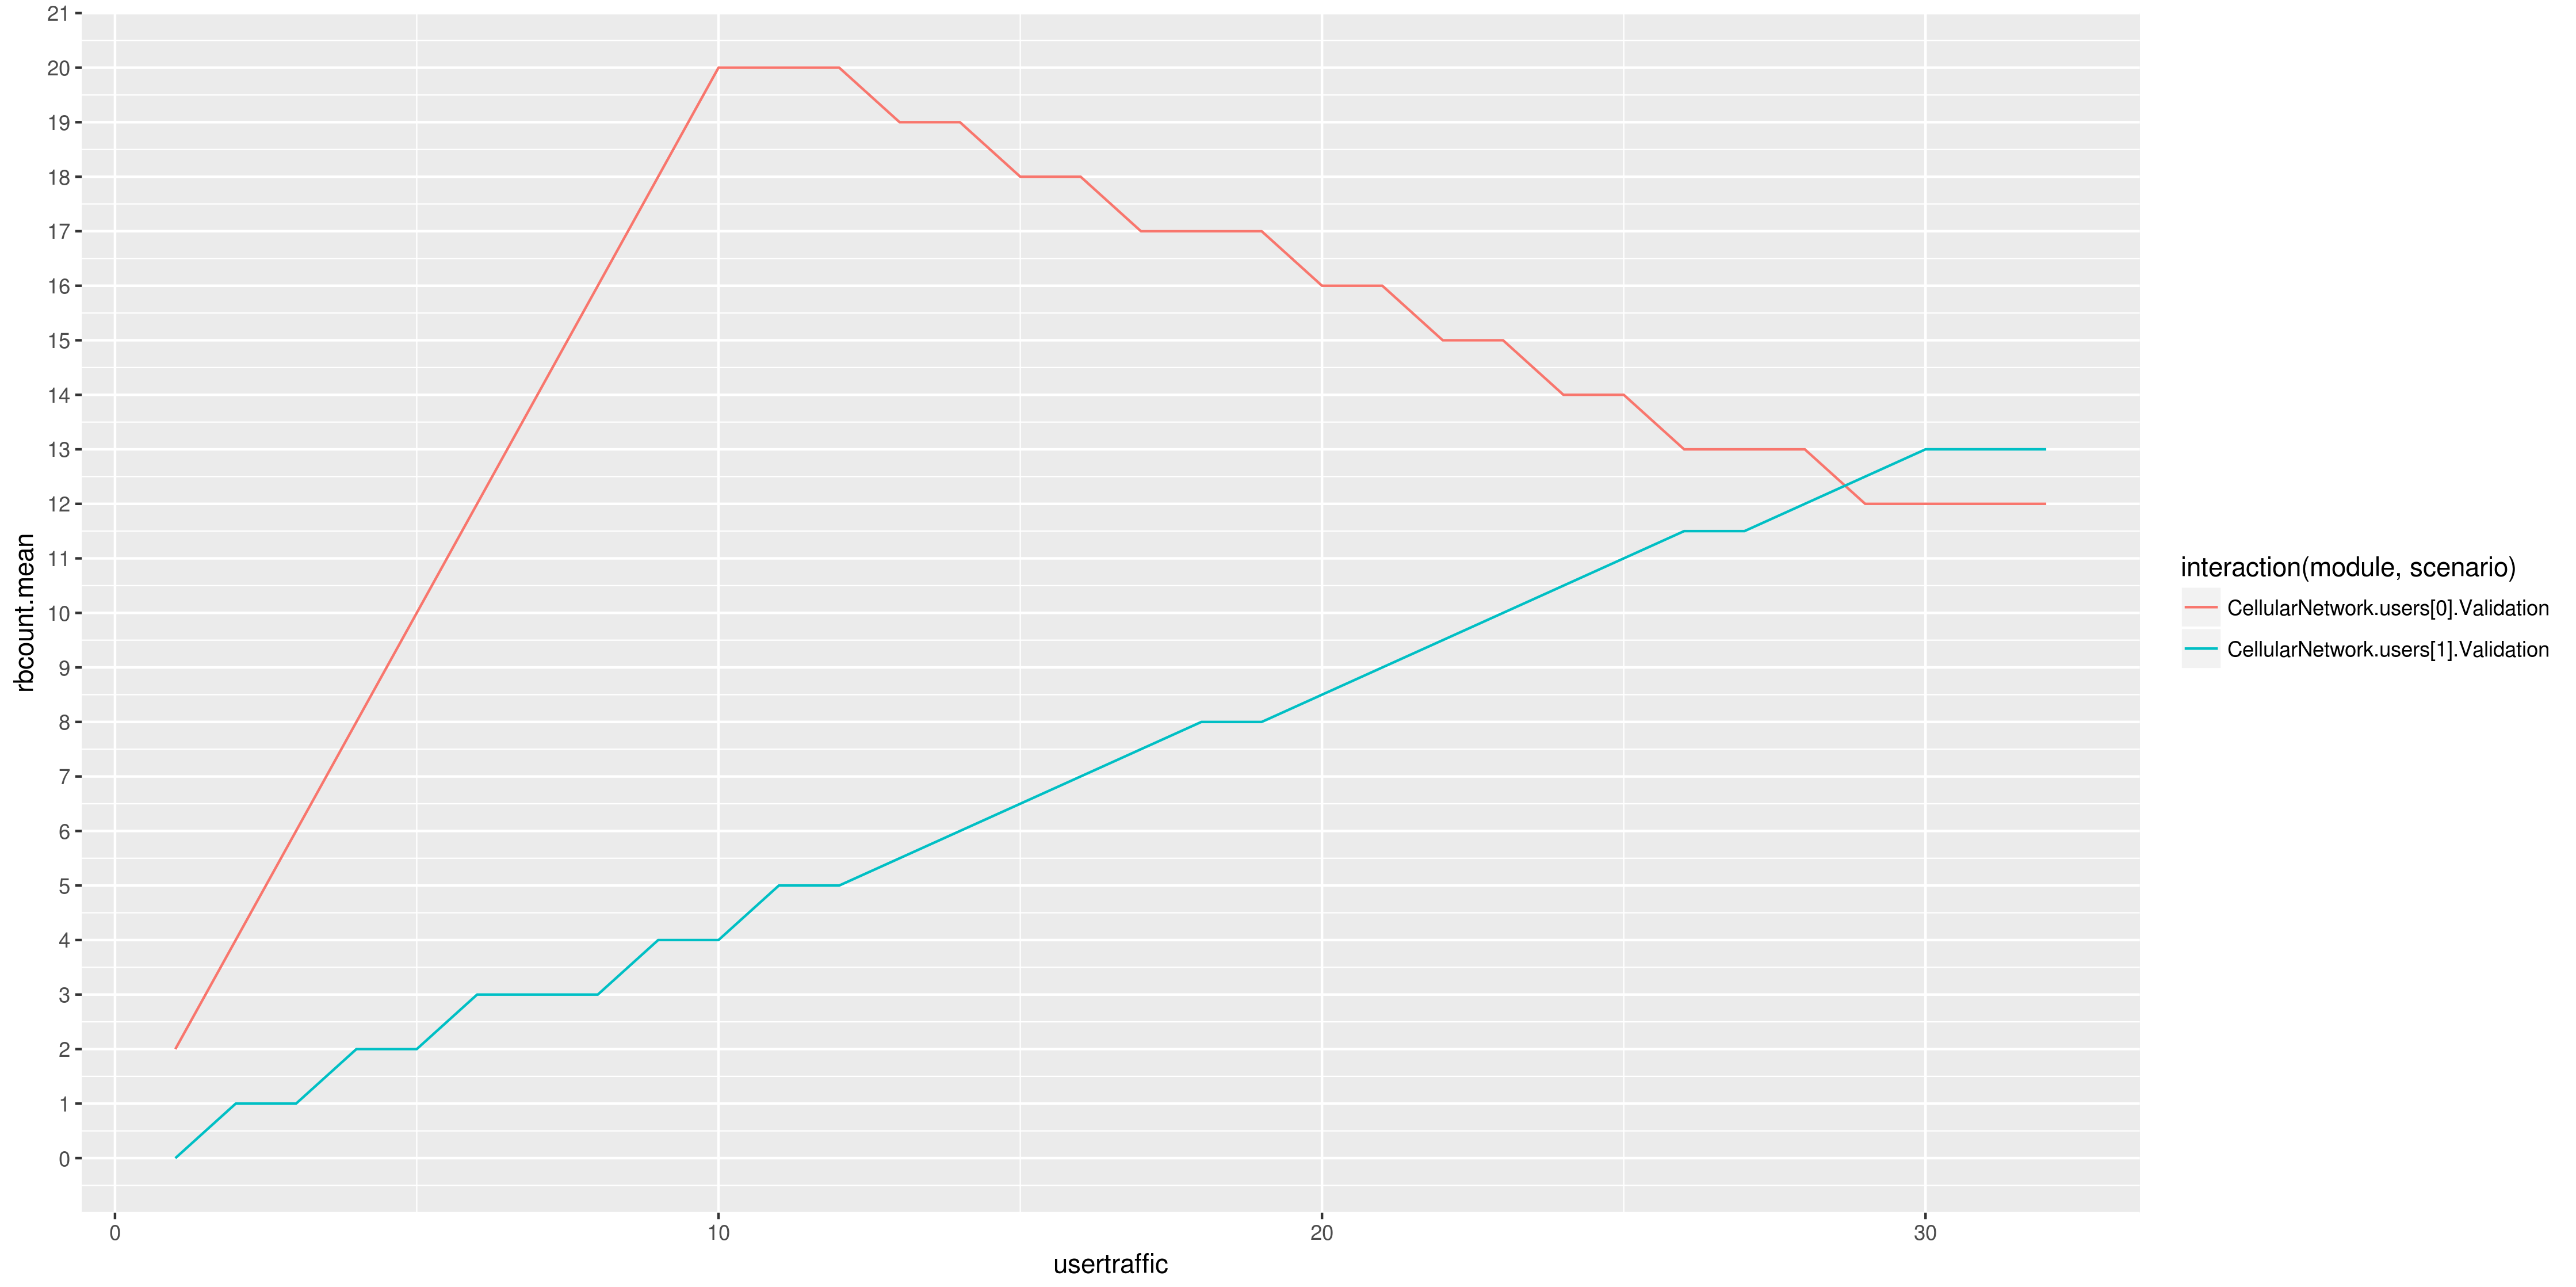
\includegraphics[width=1\textwidth]{images/RBCompvalidation2}
  \caption{2nd validation scenario: mean RB count}
  \label{fig:2nd validation scenario: mean RB count}
\end{figure}
By math the mean RB would be \(\#RB / 2 = 12.5 \) but the number of RB assigned per user is slightly different since, on average, 12 RBs are assigned to \texttt{Mobile User[0]} and 13 RBs are assigned to \texttt{Mobile User[1]}. This oddness is due to fragmentation of packet. In our simple model infact packets can not be fragmented so if a packet does not fill inside the last RB this RB is lost and it assigned to the next user. Note that in validation scenarios everything is fixed, also packet dimension, so there could be strangeness like that. However we can say that our model is quite accurate and can be used to simulate the network in more complex scenarios. 
There is another strange behavior that involves response time. When the input traffic is too high we expect that response grows indefinitely since packets get queued. However, by observing the graph, the mean response time seems to approch to \(ST/2\). In the following graph it is displayed the response time of packets addressed to \texttt{Mobile Station[0]} when the rate \(\lambda = 40\), so it is very high.
\begin{figure}[H]
  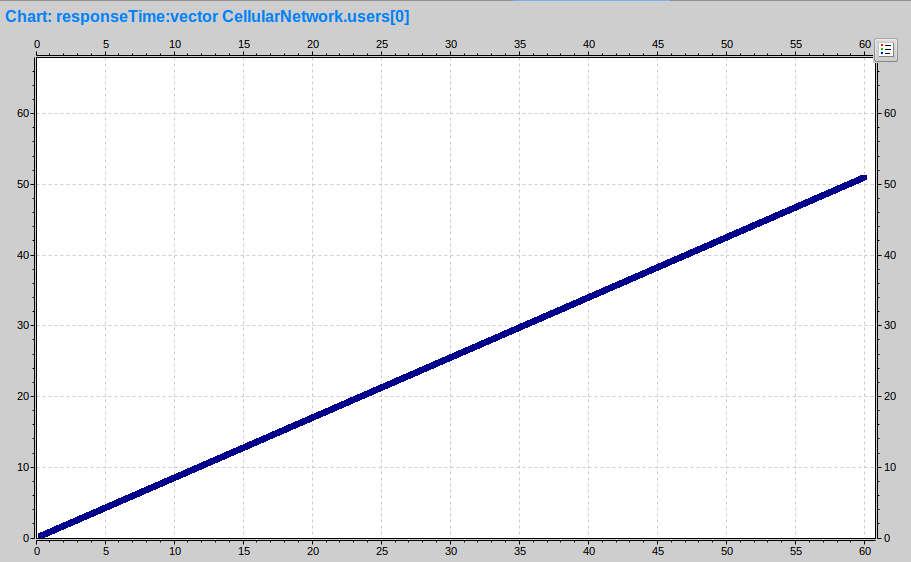
\includegraphics[width=1\textwidth]{images/response-timeVec}
  \caption{2nd validation scenario: response time(vector)}
  \label{fig:2nd validation scenario: response time(vector)}
\end{figure}
We we can see cleary a linear relation between simulation time and response time when the system is unstable. We can describe the relation as:
\begin{equation} 
	RT(t) \approx \frac{\max(RT)}{ST}t, \quad 0\le t \le ST 
\end{equation}
The previous formula has that meaning: \textit{a packet which is generated at time t will have a response time about equal to \(RT(t)\)}. Now we can try to calculate the \textit{mean response time}.
\begin{equation}
\begin{split}
E[RT(ST)] &= \frac{\sum\limits^{ST}_{t=0} RT(t)}{ST} = \frac{\sum\limits^{ST}_{t=0} \frac{\max(RT)}{ST}t}{ST} = \frac{\max(RT)}{ST^2}\sum\limits^{ST}_{t=0}t =
	\\ &= \frac{\max(RT)}{ST^2}\frac{ST(ST+1)}{2} = \frac{\max(RT)}{2}\frac{ST+1}{ST} \approx \frac{\max(RT)}{2}
\end{split}
\end{equation}
At the end we can observe that if the system is unstable \(RT(t)\) has a linear behavior so if we calculate the mean at the end of simulation we obtain \(E[RT(ST)] \approx ST/2\). 


\section{3\textsuperscript{rd} test: NoFramingTest, uniform CQI, exponential interarrivals, fixed packet size, 10 users}

This is a test to validate eventually the model shown in the previous chapter. It's too difficult to build a full matematical model starting from the requirements, but having no one is not helpful in explaining the simulation results. So we started to build simple models by leaving off some of the requirements and by considering only some specific conditions (like saturation). In our case one of the most difficult things to model is \textit{frame sharing}.
As the requirements said, we have two \textit{packet allocation policies} to implement: if a packet cannot completely fill the frame, it cannot be scheduled and the scheduler moves to the next user. Furthermore, every RB cannot contain packets from two or more different users. This means that there will be some wasted space to consider.
The first policy is what causes \textit{frame sharing}, because some totally free RB are used to empty to serve di other users.

A question now arises: how this packet allocation policies will influence our results? Intuition make us think that total antenna throughput will get somewhat worse, just thinking about the wasted space.
To confirm this intuition we set up another scenario, called NoFramingTest, which will be running using the following parameters:

\begin{itemize}
	\item \(\#users = 10\)
	\item \(CQI_i \sim U(1,15)\)
	\item \(packetsize_i=25 \textnormal{ B}\)
	\item \(interarrivalrate_i \sim exp(\lambda)\)
\end{itemize}

The most strange parameter here is \(packetsize\). This is a simple way to have no frame sharing at all in our simulation. We could end up fixing \(packetsize=1 \textnormal{ B}\), which would be the simplest way, however simulation would be too heavy to run at higher traffic rates (we tried, but our PCs started frying). Recalling that we need just to check throughput in saturation, we can suppose that every frame is only filled with packets from the currently selected user (using RR policy).
Studying the formula that defines the total frame size of each client in our model:
\begin{equation}
	\begin{split}
	&rbsize_i = f(CQI_i) \\
	&framesize_i = \#RB \times rbsize_i
	\end{split}
\end{equation}
The number of packets that will fill the frame can be computed as:
\begin{equation}
\#packets_i = framesize_i/packetsize
\end{equation}
where \(packetsize\) is fixed, our goal is to find a \(packetsize\) such that \(\#packets_i\) is a natural number (all packets fill exactly the frame) for each client (\(i\)).
As we said, \(packetsize=1\) is a solution, however another interesting solution is \(packetsize=25\). This is due to the fact the \(\#RB=25\) is fixed and used to compute every client frame size. Note that this is valid only if frame is filled every time by a single client (as the previous assumption).
Lets check the throughput results:
\begin{figure}[H]
  \includegraphics[width=1\textwidth]{images/{all-nofram}.png}
   \caption{No-framing scenario: throughput, response time}
  \label{fig:all-nofram}
\end{figure}

First let's make sure that no \textit{frame sharing} happens at the higher throughput rates:
\(lambda_{sat}\) is at about \(4.1\) and we can see from the next graph that there is no \textit{frame sharing} at all over that rate! This graph measures basically how many RBs are shared to users other than the current served user.
\begin{figure}[H]
  \includegraphics[width=1\textwidth]{images/{fillrb-nofram}.png}
   \caption{Mean nfill graph, NoFramingTest scenario}
  \label{fig:fillrb-nofram}
\end{figure}\
Note that for \(\lambda_i < \lambda_{sat}\) \textit{frame sharing} is still present because \(nfill > 0\) and that is what we expected.

Now we can extract the throughput at \(\lambda_{sat}\), which is \(8127675 \pm 13109\ bit/s \simeq 8.128 \pm 0.131\ Mbit/s\).
%th_confmin 8114566
%th_mean:   8127675 +- 13109
%th_confmax 8140784

A simple mathematical model to compute antenna total throughput can be:
\begin{equation}
	E[th_{antenna}] = \frac{\sum\limits_{i=1}^{\#client} \#RB \times E[rbsize_i]}{\#client\times(1/T_{slot})} = \frac{\sum\limits_{i=1}^{10} 25 \times E[rbsize_i]}{10 \times (1/T_{slot})}
\end{equation}
\(rbsize_i\) is a RV variable with an unknown distribution, however
\begin{equation}
	 rbsize_i = f(CQI_i), \quad CQI_i\sim intU(1,15), \quad \forall i \in [1,10]
\end{equation}
This means we can simply use the general formula for functions of RVs
\begin{equation}
	E[X] = \sum_{x_i : g(x_i)=y_i}^{} g(x)p(x) = E[g(x)]
\end{equation}
Considering that
\[f(cqi) = [3,3,6,11,15,20,25,36,39,50,63,72,80,93,93] \]
our result, that will be used also in other computations, is
\begin{equation}
	E[rbsize_i] = \frac{1}{15} \times \sum_{cqi=1}^{15} f(cqi) = 40.6 \textnormal{ B}, \quad \forall i \in [1,10]
\end{equation}
which is constant for all clients. In this case the initial model can be simplified to
\begin{equation}
E[th_{antenna}] = \frac{\#RB \times E[rbsize_i]}{1/T_{slot}} \times 8 = 8.12 \textnormal{ Mbps}
\end{equation}
The mean \textbf{matches} the throughput simulated result!

This test is not only for a validation purpose, but it is a starting point to study how frame sharing impacts network performances. We will see this later.
\chapter{Simulation: Uniform Scenarios}
\section{Introduction}
In this chapter we will consider \texttt{Mobile Stations} which, at each timeslot, generate CQIs with an integer uniform distribution. In the validation scenario we proved that scheduler is fair so we expect that all users will have similar values for the mean throughput and the mean response time. In this simulation we will consider the following parameters:
\begin{itemize}
	\item \(n=10\)
	\item \(packetsize_{i} \sim U(3,75), \quad 0 \le i \le n-1\)
	\item \(CQI_{i} \sim U(1,15), \quad 0 \le i \le n-1\)
	\item \( \lambda = \lambda_{i} = 0.1 + 0.5k, \quad k\in\{1,2\ldots,10\}, \quad 0 \le i \le n-1\)
\end{itemize}
This scenario is almost similar to the NoFraming Validation test, but the main difference is that \(packetsize\) is a uniform RV. As we said before we expect to get worse throughput result due to the fact that some RB space will be left empty because packets cannot be fragmented. 

We will simulate the scenario with both scheduler and we will check if our first intuition is true or not and the impact of \textbf{framing} in the average performance metrics.

\section{Uniform CQI, Fair Scheduler}
In this simulation we will consider the basic \textbf{Fair Scheduler}. We remember that, in this case, if \(currentUser\) empties his queue or has a packet that is bigger than \(RB_{size}\) the scheduler will consider the next users.

\begin{figure}[H]
  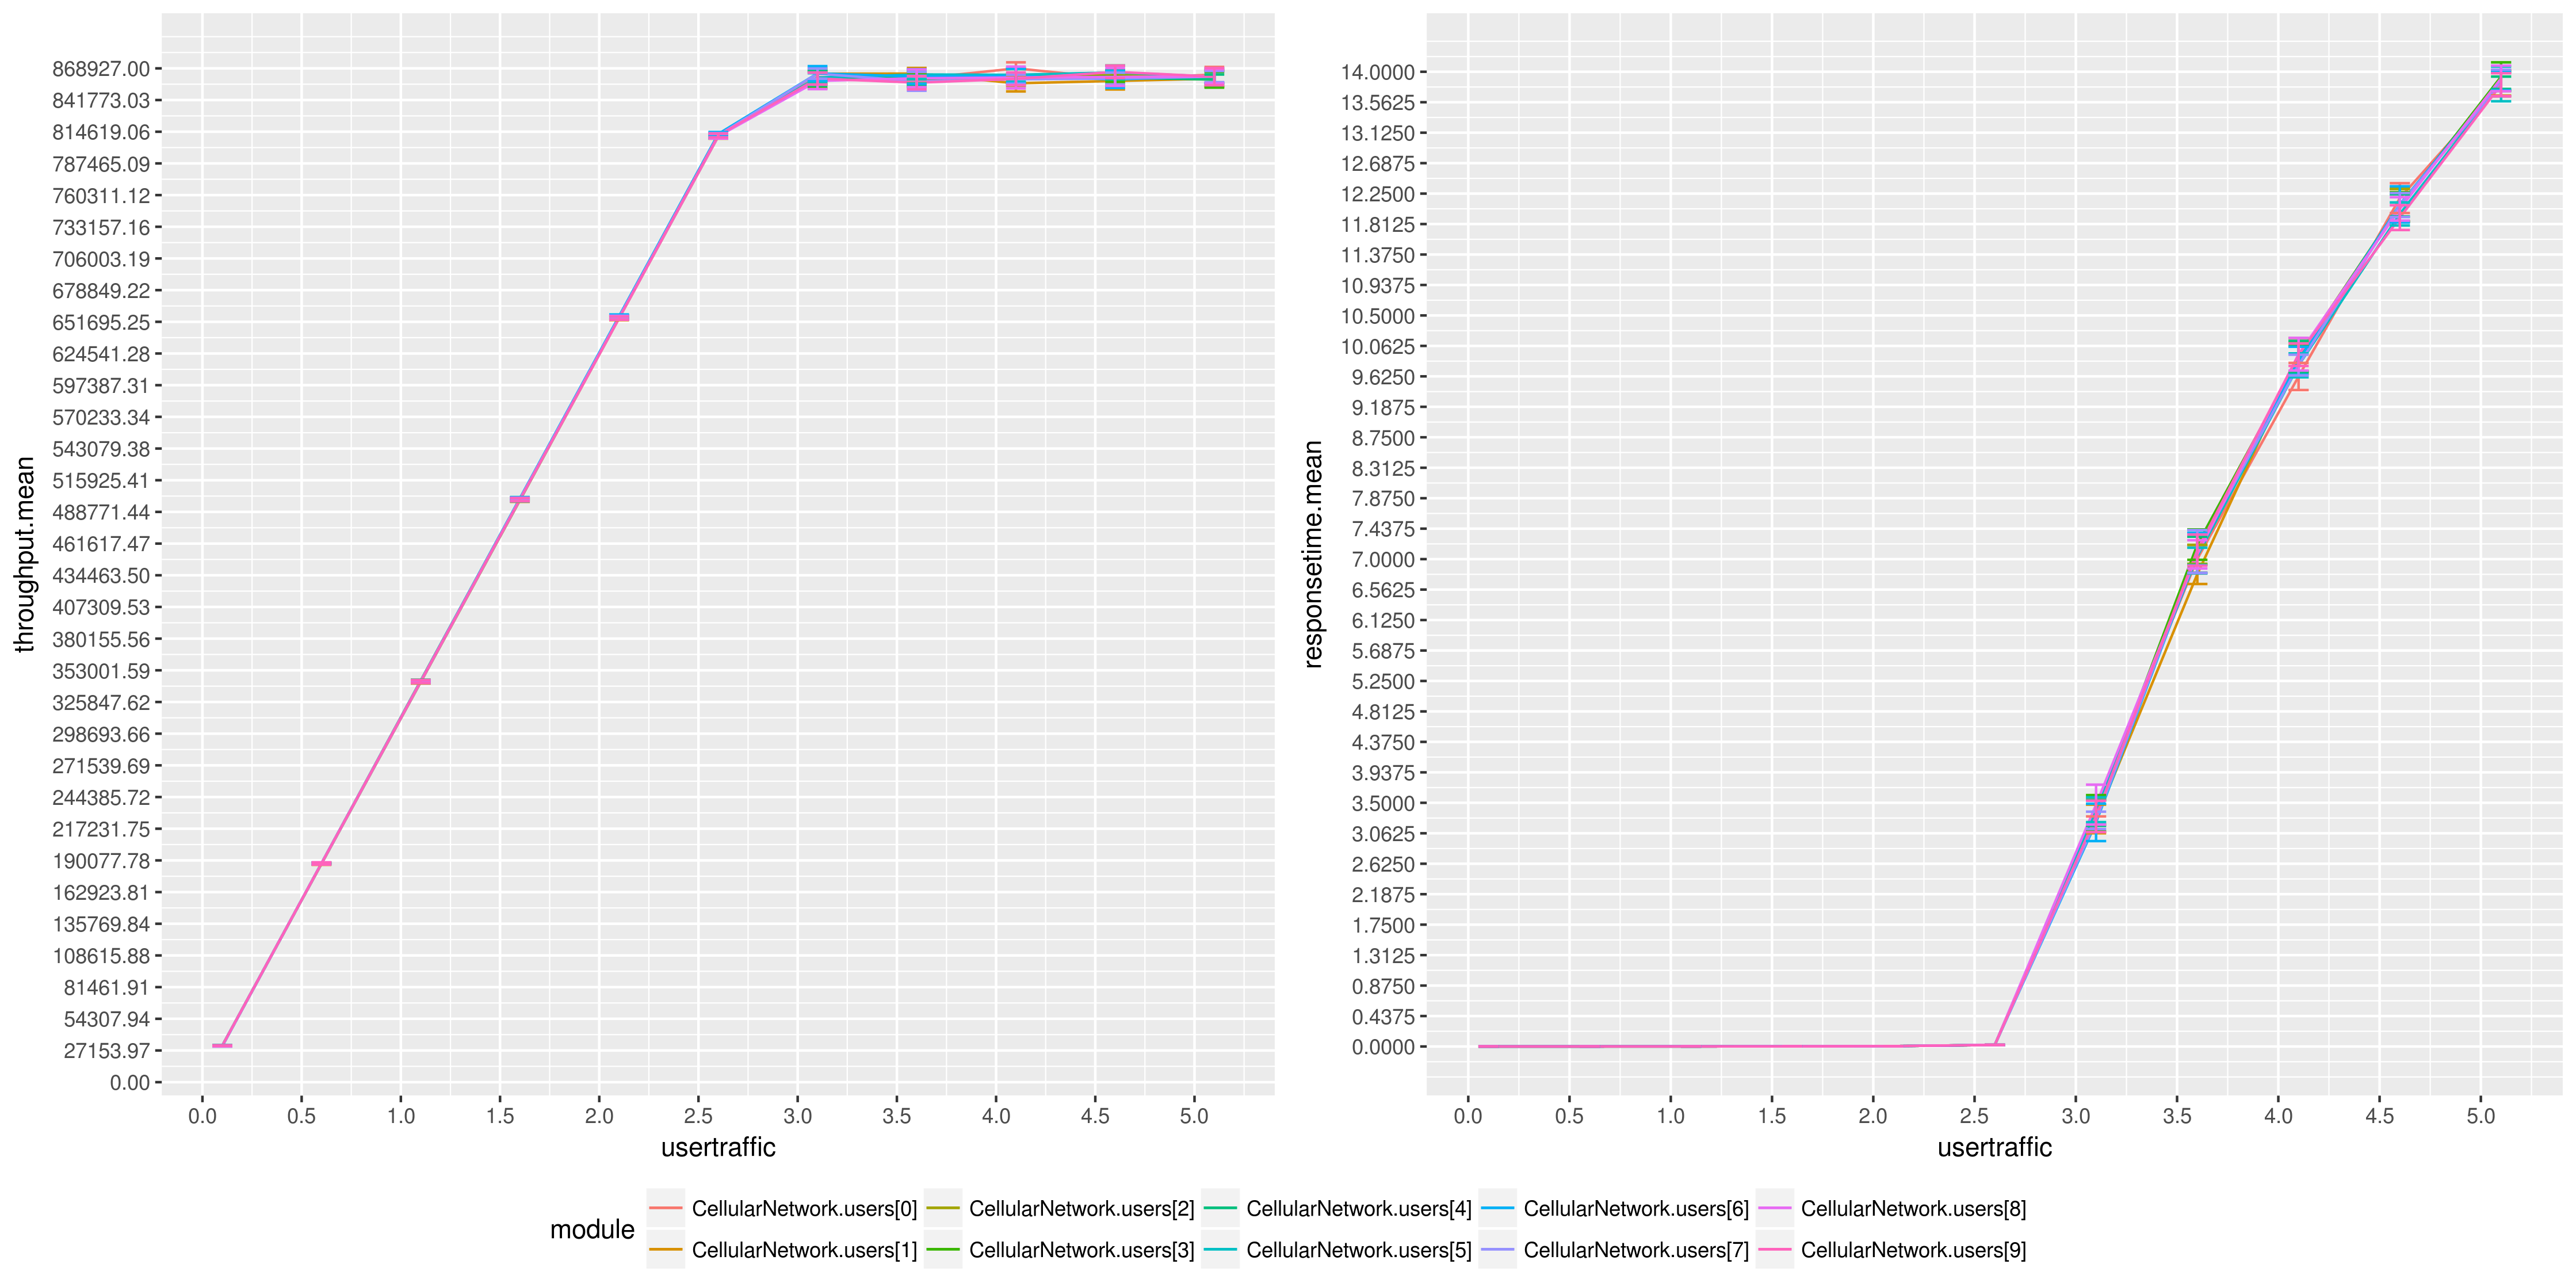
\includegraphics[width=1\textwidth]{images/unif}
  \caption{uniform scenario: throughput, response time}
  \label{fig:uniform scenario: throughput, response time}
\end{figure}
The first thing we can notice is that every client has the same saturation point (which depends on \(\lambda\)): this can be explained considering that scheduler is fair and every client generates, on average, the same amount of packets (which are also the same size on average). Response times are stable before reaching the common saturation point and after tends to arise indefinitely, until reaching a maximum. This maximum is the same shown in the \(2_{nd}\) Validation test and has the same explaination. So the only valid values for Response Times are generated between \(0 < \lambda < \lambda_{sat}\), which is common for each client. 

In the graph we notice that \(\lambda_{sat}=3.1\). If we compare this rate with the maximum rate computed in the 1\textsuperscript{st} Validation Test we observe that \(\lambda_{sat} = \lambda_{max}/10\). This is not surprising since there are 10 \texttt{Web Server} wich push traffic to the Antenna. Each one is a \textit{Poisson process} with rate \(\lambda\) so the superimposition of 10 them is a \textit{Poisson process} with a rate \(\Lambda = 10\lambda\). Actually the system saturates before \(\lambda=3.1\), infact in validation we considered the best case where \(CQI=15\) so RBs had the maximum size. Here \(RB_{size}\) is a RV however \(\lambda_{sat}=3.1\) is a raw approximation confirmed by the results of the simulation.

The most important result, here, is the antenna total throughput. Lets see:
\begin{figure}[H]
  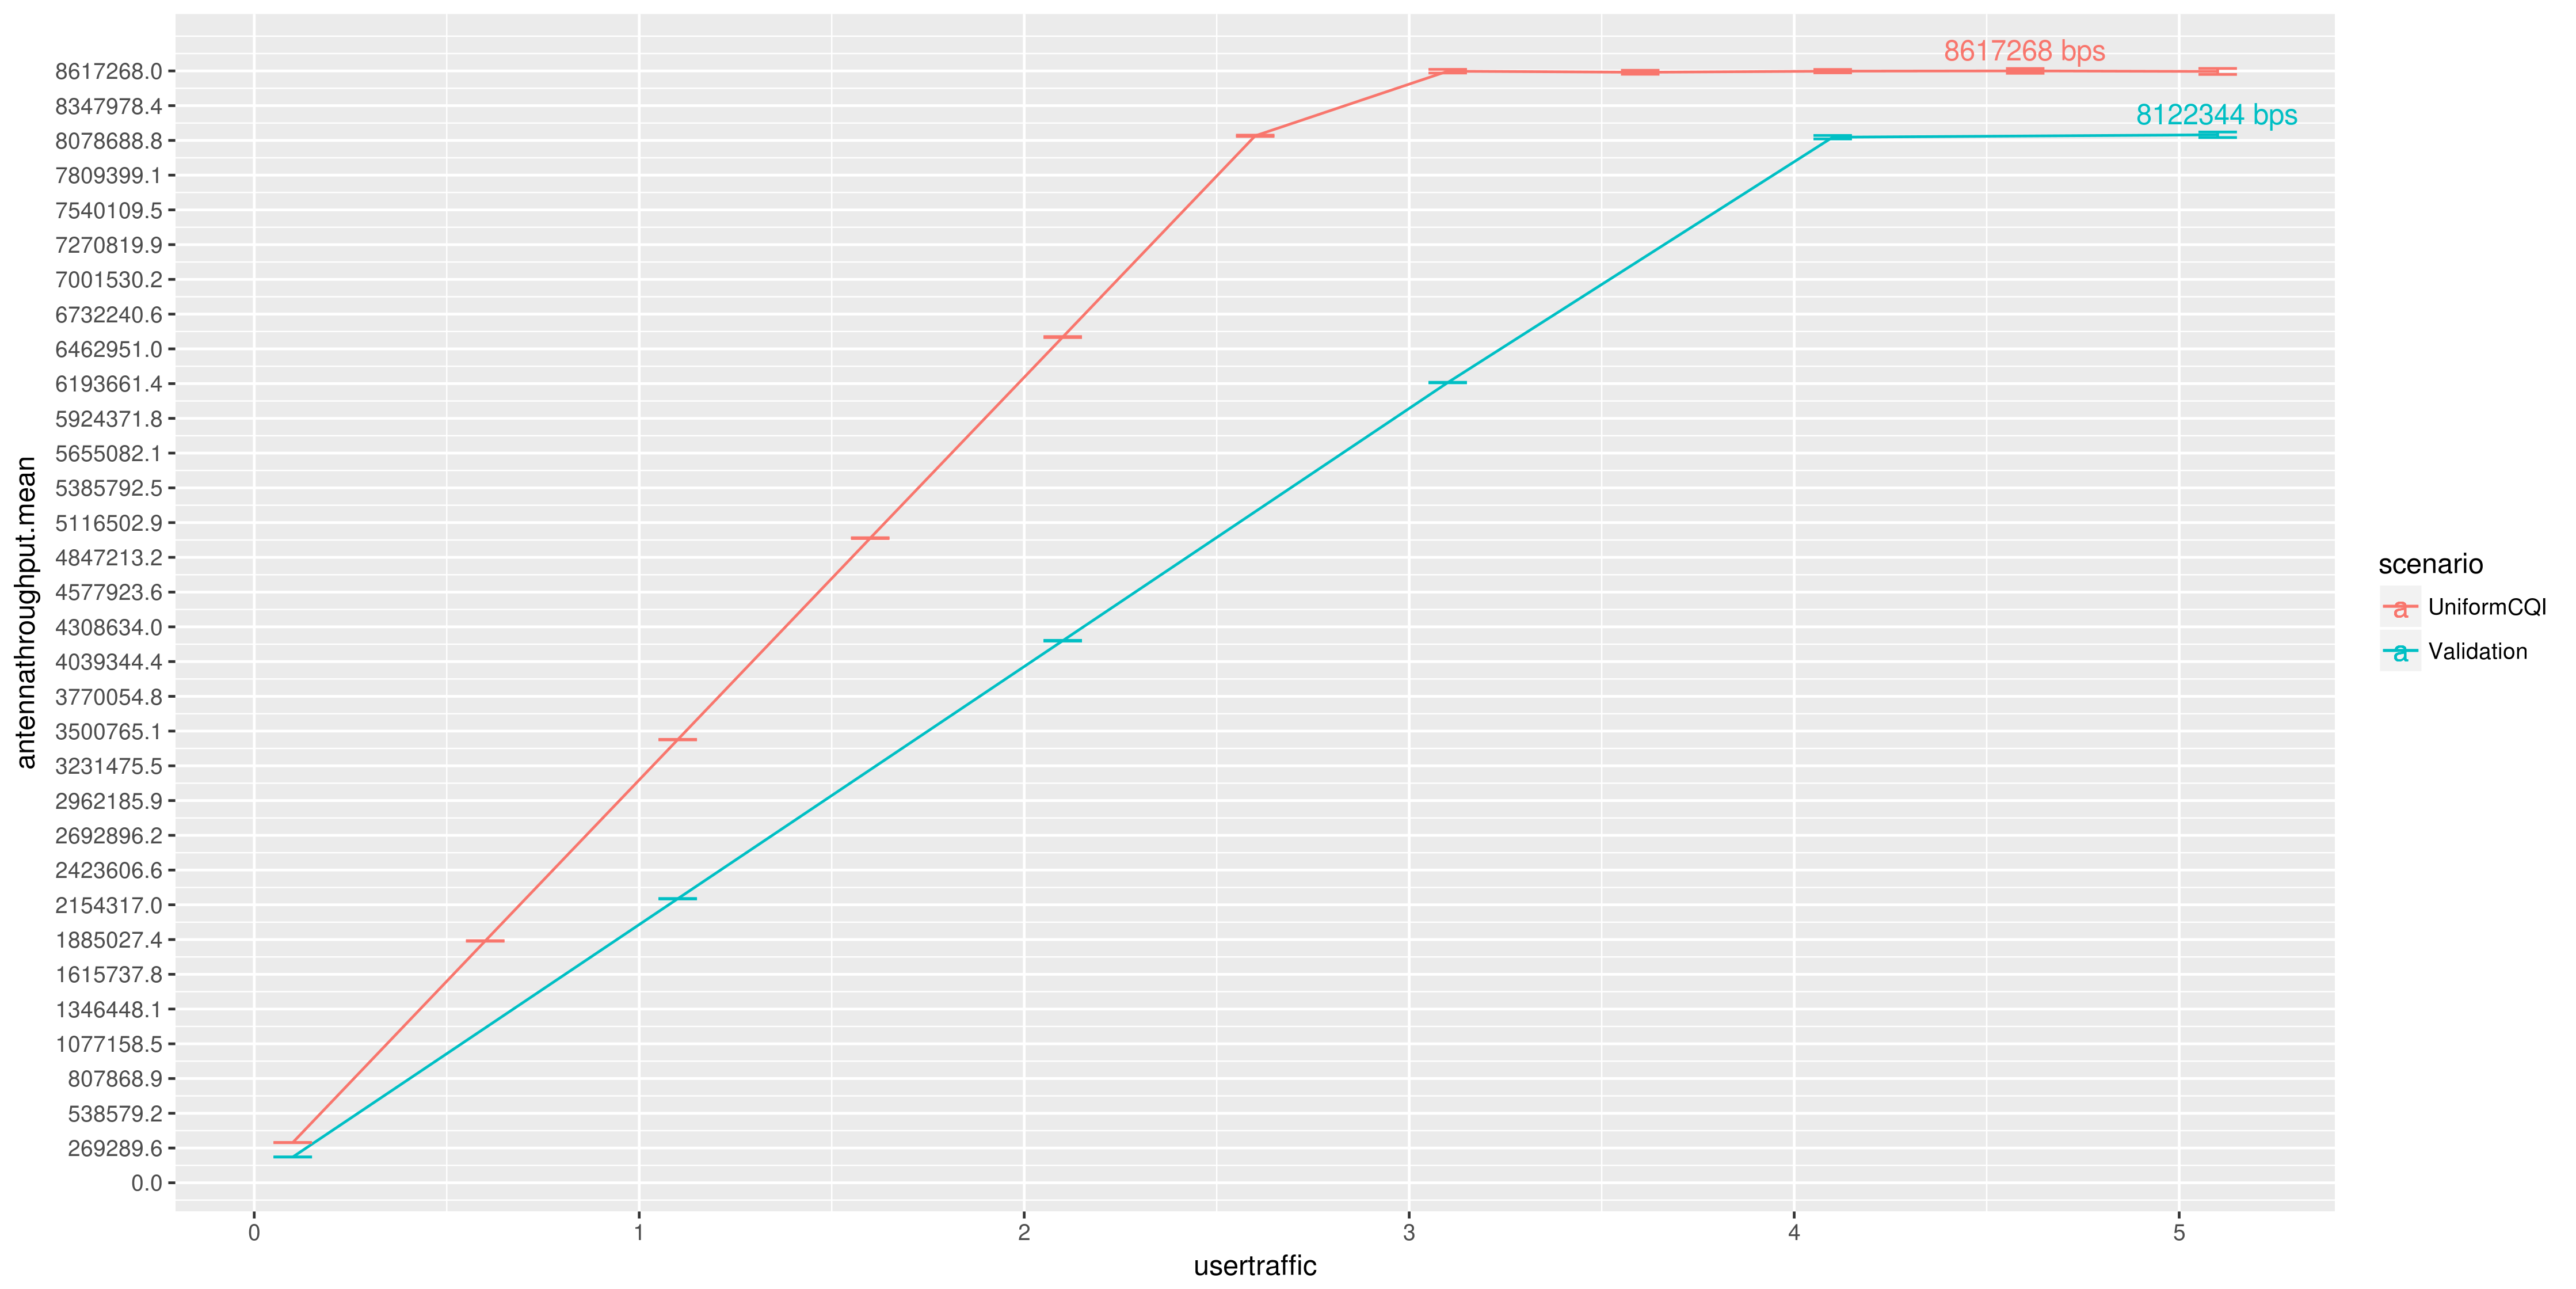
\includegraphics[width=1\textwidth]{images/thantenna1}
  \caption{Antenna throughput: UniformCQI, Validation-NoFramingTest}
  \label{fig:Antenna throughput: UniformCQI, Validation-NoFramingTest}
\end{figure}

Comparing to the 3\textsuperscript{rd} NoFraming Validation test result, our global throughput is \textbf{higher}. This is a very very strange result that \textbf{destroys our first intuition} about the impact of framing.

How can the throughput get higher? Thinking about our model, we came up with a possible explanation. Framing policies, as we seen before, are basically two:
\begin{itemize}
	\item One RB cannot contain traffic from 2 or more different clients
	\item If a packet cannot entirely fit the frame, it cannot be scheduled
\end{itemize}
The first policy cannot give us an higher throughput and this is already proven: we are telling that some frame space is eventually wasted, and this leads always to a worse or equal throughput result. So lets focus on the second policy: our intuition (hopefully correct this time) suggests us that framing, as a measure of how much RBs are not filled due to framing, is uniformly distributed for each client. Lets remember that the remaining space is allocated to other clients using a Fair policy (FairScheduler) and \(framesize_i\) depends on \(rbsize_i = f(CQI_i)\). Now lets try to analyze a single iteration of the scheduler algorithm, applied to 2 clients in the following state:
\begin{align}
 \#RB_{free} &= 1, &currentUser &= 1 \nonumber \\
 	   CQI_1 &= 1, &rbsize_1 &= 3 \nonumber \\
	   CQI_2 &= 13, &rbsize_2 &= 80 \nonumber
\end{align}

Both have one packet of \(packetsize=75\) (which is the maximum we can have) in backlog. The first client cannot fit his packet into the frame chunk, so remaining RBs (in our case just 1) are allocated to the client 2, which can now fit his packet into his frame chunk. The main factor, here, is \(framechunksize_i = remainingRBfor_i \times rbsize_i\): we are telling that client with the best CQI can fit more likely his packets into the frame, despite of the current serving user, due to the fact that his \(framechunksize_i\) is bigger than the other clients. This reminds us a bit of BestCQI Scheduler policies.

However we must consider that the previous case does not describe completely all the possible behaviors of the system. Infact, lets consider this other case:
\begin{align}
	\#RB_{free} &= 1, &currentUser &= 1 \nonumber \\ 
	CQI_1 &= 3, &rbsize_1 &= 6, & backlog &= \textnormal{1 packet of 75 bytes} \nonumber \\
	CQI_2 &= 1, &rbsize_2 &= 3, &backlog &= \textnormal{1 packet of 3 bytes} \nonumber \\
	CQI_3 &= 13, &rbsize_3 &= 80, &backlog &= \textnormal{1 packet of 75 bytes} \nonumber 
\end{align}

Client 1 packet cannot be scheduled (\(75 > 6\)), so we go next to the second user which can now fit his packet into the new frame chunk (3 = 3). As we can see here, the RB is allocated to the user with the worst CQI (client 2) and not the best (client 3). So we can also deduce that a client with a small packet in backlog is more likely to fit his packet into the frame.

Combining this result with the previous we can infer that a packet is more likely to fit if:
\begin{itemize}
	\item The packet is small
	\item The user CQI is high
\end{itemize}
We can add another case:
\begin{align}
	\#RB_{free} &= 1, &currentUser &= 1 \nonumber \\
	CQI_1 &= 3, &rbsize_1 &= 6, &backlog &= \textnormal{1 packet of 75 bytes} \nonumber\\
	CQI_2 &= 1, &rbsize_2 &= 3, &backlog &= \textnormal{1 packet of 75 bytes} \nonumber\\
	CQI_3 &= 2, &rbsize_3 &= 3, &backlog &= \textnormal{1 packet of 75 bytes} \nonumber
\end{align}
None of the packets cannot be inserted into the framechunk, so the RB is completely wasted. This is the case that lowers the throughput, due to the fact that packet sizes are small and CQIs are low. However, in our scenarios (Uniform, UniformBest, Binomial ...) the number of users is high enough (10 users) to get, more likely, at least a small packet and/or at least a good enough CQIs to not waste the remaining space.

%At the end we can see that this result lies between \textit{NoFramingTest} and \textit{Uniform BestCQI} results: in fact ``The user CQI is high'' is the main policy of BestCQI scheduler. However, in that scenario, we can't consider ``The packet is small'' because BestCQI user is \textbf{always} selected as first for the residual frame filling, and this increases the throughput for BestCQI scenario.

%CQIs and packet sizes are always uniform for all clients, so we suspect that all clients will benefit of a small and equal throughput increase.
%\begin{center}
%	INSERIRE IMMAGINE QUI ALLTH NOFRAMINGTEST EVENTUALMENTE, magari confrontare il test con quelli dell'uniform e far vedere che i throughput sono più bassi in NoFrameFilling
%\end{center}
%\

Note that we have tried to analyze just few cases and do a very raw approximation of antenna total throughput mean value tendency, so we can't make an exact model of the system in order to proof this result analytically. 
At the end of simulation we can summarize these results about the Uniform Scenario with Fair Scheduler:
\begin{itemize}
	\item Saturation rate \(\lambda = 3.1\)
	\item Antenna throughput \(th_{antenna} = 8615055 \pm 14206 \textnormal{ bps}\), \textit{conf lvl 95\%}
	\item User throughput \(th_{i} = 861343 \pm 4968 \textnormal{ bps}\), \textit{conf lvl 95\%}
\end{itemize} 

\section{Uniform, Best CQI scheduler}
Now we will simulate the scenario by using the second scheduler. If there were not \textbf{framing} the performance of both scheduler would be the same but, as seen before, \textbf{framing} is present and has a great impact in performance. We can expect this scheduler will have better performance in throughput since it fills the residual space inside the frame by using packets addressed to users with higher CQIs.
\end{document}